\documentclass[12pt,fleqn]{article}\usepackage{../../common}
\begin{document}
Materyel Mekaniği - 5

Bükülen bir çubuğun formüllerine bir giriş [1] kaynağında yapıldı. Orada
moment-eğri (moment-curvature) formülü gösterilmişti. Şimdi bu formüle
farklı bir yerden eriselim ve onu ikinci derece türeve eşitleyelim.

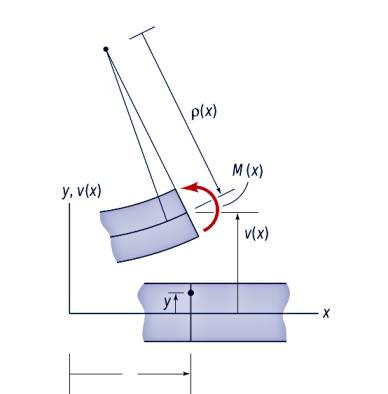
\includegraphics[width=10em]{phy_020_strs_05_01.jpg}

Resimde gösterilen semboller $M$ bükme momenti, $\rho$ çubuğun $+y$ tarafındaki
bükülme çemberinin, eğiminin yarıçapı (radıus of curvatüre).  $v$ ise yine $+y$
kısmındaki yer değişimidir. Çubuğa uygulanan kuvvet dağılımının ne olduğu
önemli değil, sonuçta odaklandığımız çubuğun ufak bir kısmı

[4] kaynağında bir çemberi (yarıçapını) onun bir eğriye dokunduğu noktadaki
türevler üzerinden temsil etme tekniğini paylaştık. Bu formülü mevcut probleme
uygulayabiliriz.

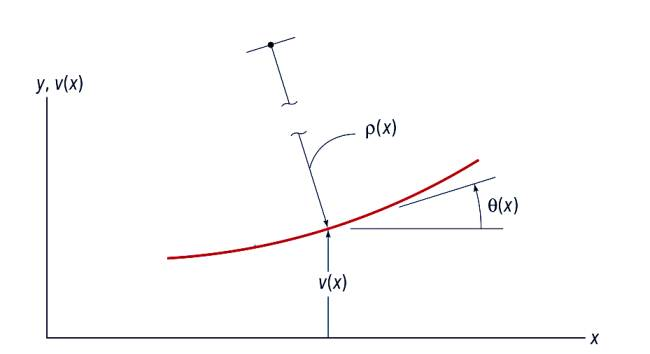
\includegraphics[width=20em]{phy_020_strs_05_02.jpg}

Bu ilişki

$$
\frac{1}{\rho} =
\frac
{\dfrac{\ud^2 v}{\ud x^2}}
{ \left[ 1 + \left( \dfrac{\ud v}{\ud x}  \right)^2 \right]^{3/2} }
$$

Ustteki problemde eğim çok ufaktır o zaman $\ud v / \ud x$ ufak kabul edilir
(resimdeki eğim eğitim amaçlı abartılmış), demek ki bolendeki kare hesabi
daha da ufalir, geriye sadece 1 kalir, 1 ile bolumu yok sayariz, geriye kalanlar

$$
\frac{1}{\rho} \approx \frac{\ud^2 v}{\ud x^2}
$$


Kaynaklar

[1] Bayramlı, {\em Fizik, Materyel Mekaniği - Hazırlık}

[2] Craig, {\em Mechanics of Materials, Third Edition}

[3] Bayramlı, {\em Çok Değişkenli Calculus, Eğrilik (Curvature)

\end{document}
